\begin{figure}[H]
\centering
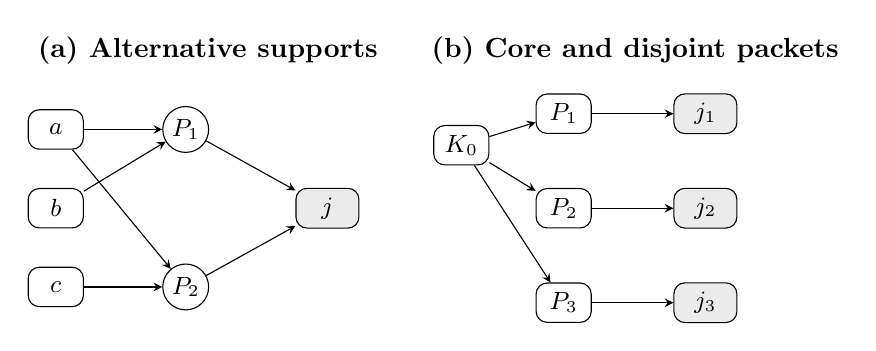
\begin{tikzpicture}[font=\small,source/.style={draw,rounded corners,minimum width=7mm,minimum height=5mm},proof/.style={draw,circle,inner sep=1.5pt},goal/.style={draw,rounded corners,fill=black!8,minimum width=8mm},edge/.style={->,>=stealth,thin}]
\node[anchor=west,font=\bfseries] at (0,2.0) {(a) Alternative supports};
\node[source] (a) at (.35,1) {$a$}; \node[source] (b) at (.35,0) {$b$}; \node[source] (c) at (.35,-1) {$c$};
\node[proof] (p) at (2,1) {$P_1$}; \node[proof] (q) at (2,-1) {$P_2$}; \node[goal] (j) at (3.8,0) {$j$};
\draw[edge] (a)--(p);\draw[edge] (b)--(p);\draw[edge] (a)--(q);\draw[edge] (c)--(q);\draw[edge] (p)--(j);\draw[edge] (q)--(j);
\node[anchor=west,font=\bfseries] at (5,2.0) {(b) Core and disjoint packets};
\node[source] (k) at (5.5,.8) {$K_0$};\node[source] (r) at (6.8,1.2) {$P_1$};\node[source] (s) at (6.8,0) {$P_2$};\node[source] (t) at (6.8,-1.2) {$P_3$};
\node[goal] (u) at (8.6,1.2) {$j_1$};\node[goal] (v) at (8.6,0) {$j_2$};\node[goal] (w) at (8.6,-1.2) {$j_3$};
\draw[edge] (k)--(r);\draw[edge] (k)--(s);\draw[edge] (k)--(t);\draw[edge] (r)--(u);\draw[edge] (s)--(v);\draw[edge] (t)--(w);
\end{tikzpicture}
\caption{Support topology determines acquisition behavior. In (a), the arrow pairs into each proof node mean conjunction, while the two proof nodes are alternatives for authorizing $j$; $a$ is shared. In (b), each region needs the common core and one disjoint packet. The drawing is schematic, not a measured instance.\label{fig:support}}
\end{figure}
